\documentclass[pdftex,11pt,a4paper]{article}
\usepackage{blindtext}
\usepackage{graphicx}
\usepackage{subfiles}
\usepackage{amsmath}
\usepackage{amsthm}
\usepackage{tikz}
\usepackage{wrapfig}
\usepackage{lscape}
\usepackage{rotating}
\usepackage{epstopdf}
\usepackage[font=small,labelfont=bf]{caption}
\usepackage{hyperref}
\hypersetup{
    colorlinks=true,
    linkcolor=blue,
    citecolor=blue
}
\usetikzlibrary{shapes.geometric, arrows}
\theoremstyle{definition}
\newtheorem{definition}{Definition}[section]
\newtheorem{theorem}{Theorem}[section]
\newtheorem{lemma}[theorem]{Lemma}
\theoremstyle{remark}
\newtheorem*{remark}{Remark}
\usepackage{amssymb}
\usepackage{amsfonts}
\usepackage{mathtools}
\usepackage{geometry}
 \geometry{
 a4paper,
 total={210mm,297mm},
 left=30mm,
 right=30mm,
 top=30mm,
 bottom=35mm,
 }
\newcommand{\defeq}{\vcentcolon=}
\newcommand{\eqdef}{=\vcentcolon}
\newcommand*{\V}[1]{\mathbf{#1}}%
\newcommand{\norm}[1]{\left\lVert#1\right\rVert}
\newcommand{\justif}[2]{&{#1}&\text{#2}}
\newcommand{\qedwhite}{\hfill \ensuremath{\Box}}
\newcommand\given[1][]{\:#1\vert\:}
\newcommand{\me}{\mathrm{e}}
\DeclarePairedDelimiterX{\infdivx}[2]{(}{)}{%
  #1\;\delimsize\|\;#2%
}
\newcommand{\Conv}{\mathop{\scalebox{1.5}{\raisebox{-0.2ex}{$\ast$}}}}%
\newcommand{\infdiv}{\infdivx}
\renewcommand{\qed}{\hfill\blacksquare}
\hyphenation{op-tical net-works semi-conduc-tor tech-no-lo-gy}


\begin{document}
\title{Learning relational structures from birdsong}
\author{Authors,~a}

\maketitle


\begin{abstract}
We infer phylo-acoustic trees (relational structures built from acoustic similarity) for over 80 bird species in the British Isles. We characterise each bird species as a Variational Bayes Hidden Markov Model trained on birdsong excerpts and then use their pairwise similarity to build a phylo-acoustic tree by running Agglomerative Hierarchical Clustering. In order to achieve this, we define similarity metrics for HMMs, hence implicitly defining a \emph{length-invariant} method to compare birdsong across different species. Additionally, we show that there is a clear community structure in the resulting phylo-acoustic trees.
\end{abstract}


\section{Introduction (500 words)}
The explosion of data in recent years has allowed scientists to gain insight in a diversity of domains. Furthermore, the widespread use of computational methods has in turn provided means of rapidly extracting conclusions from data. For example, environmental scientists have been allowed to contribute to quantify environments by means of \emph{unsupervised learning} techniques, which aim to provide insight on the hidden structures of data. Quantifying environments is crucial in order to analyse phenomena in a formal manner.
\par In this work, we tackle the problem of describing a hierarchical structure of bird species only by means of their birdsong. This mathematical representation relies only on the validity of a formal analysis framework, and hence unveils relations that go beyond empirical conclusions. This phylo-acoustic tree may further our understanding of relations among bird species in a large geographical area, and bird evolution over a large span of time. 
\par Moreover, birdsong is a rich means of communication that encapsulates behavioural patterns (such as territory defence and mate attraction or competition \cite{Berwick2013, Naguib2014}) in a regular and hierarchical fashion, as shown in figure \ref{fig_birdsong_structure}. Crucially, birdsong is learnt by repetition \cite{Berwick2013}, which implies that forced migration may push flocks to learn songs that do not necessarily come from their parents. However, given a species whose birdsong has not suffered too much from this phenomenon, it might be possible to trace back the evolutionary links of bird species. On the other hand, the loss of natural habitats (which increases forced migration) may also leave us forever with questions unanswered \cite{Marler2004}.
\begin{figure}[t]
\centering
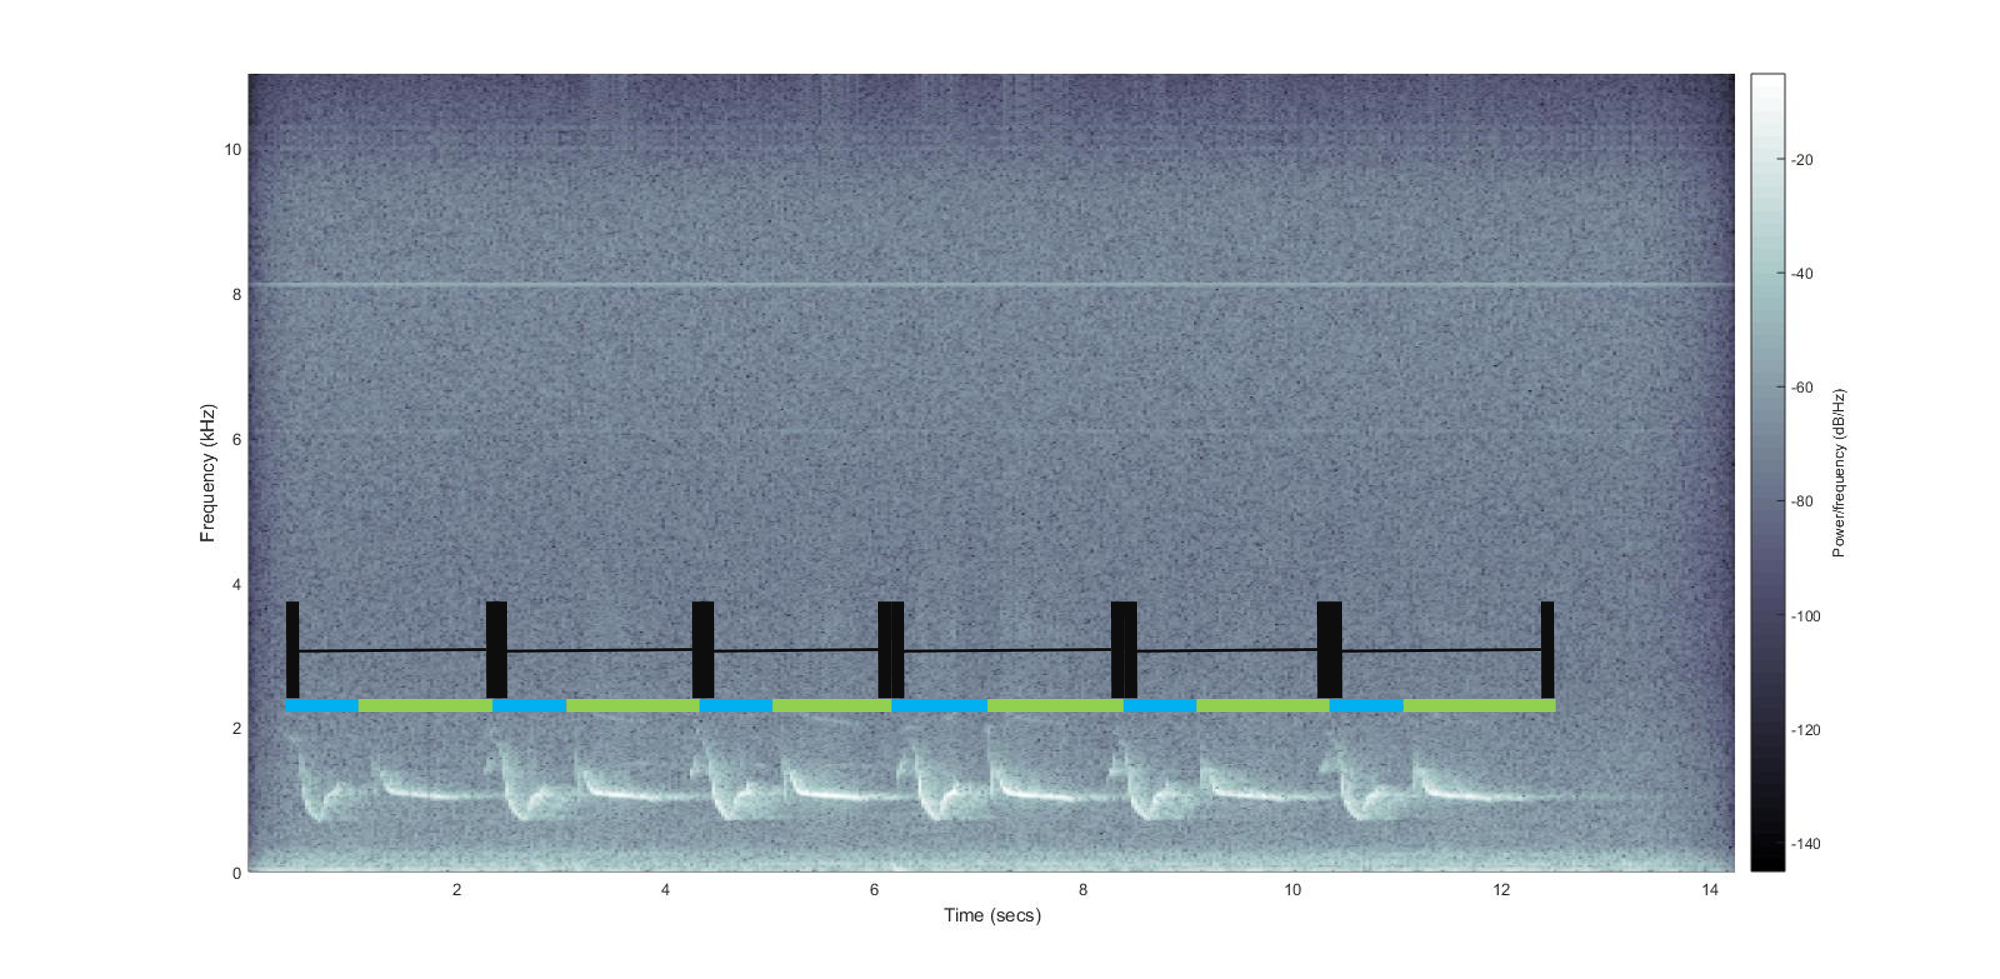
\includegraphics[width=\textwidth]{images/birdsong_structure}
\caption{Spectrogram from a birdsong recording of the species \emph{Periparus ater}. The thick blue and green bars represent syllables, and the black boxes represent a motif. Remark the pattern repeats regularly from left to right, and that motifs can be grouped hierarchically as syllables \cite{Snowdon2013}.}
\label{fig_birdsong_structure}
\end{figure}
\par Importantly, several academics in Zoology have pointed out the similarities between human speech and birdsong, e.g. we can think of both humans vowels and birdsong as ``complex, patterned vocalisations" \cite{Berwick2013,Naguib2014}. This remark enables us to analyse birdsong by means of some of the techniques from the field of Automatic Speech Recognition (ASR), which will be introduced in section \ref{section_model}. 
\par The rest of this article is organised as follows: in section \ref{section_model}, we introduce the mathematical framework used to build phylo-acoustic trees; then, in section \ref{section_results}, we present our experiments and results; and in section \ref{section_conclusion} we present our conclusions and future work.

\section{Model architecture (1500-2000 words)}
\label{section_model}
In this section, we describe the procedure to build phylo-acoustic trees given a dataset $\mathcal{D}$ with audio recordings of birdsong of different bird species from a set $X$. We are interested in finding a relation $R$ over pairs of elements in $X$, along with a scalar $s_{i, j} \in \mathbb{R}$ called the \emph{similarity} between species $x_i, x_j \in X$, i.e. $R \subseteq X \times X \times \mathbb{R}$. This relation can then be expressed as a symmetric matrix $A = (s_{i,j})$ and be used as input to build a phylo-acoustic tree by means of Agglomerative Hierarchical Clustering (AHC). 
\par Due to the continuous nature of birdsong, recordings in $\mathcal{D}$ are rarely of the same length, and hence we would like to build a similarity matrix that is \emph{length-invariant}. We achieve this by characterising each bird species $x_k \in X$ as a statistical model, and then by defining a similarity metric between pairs of statistical models. In the rest of this section, we aim to describe such similarity metrics, and then explain how they can be used in conjunction with AHC to build phylo-acoustic trees.

\subsection{Building similarity matrices}
In our approach, we associate each bird species to a probability distribution of the frequency features of their birdsong, and then compute the pairwise similarity matrix of these distributions. In order to extract frequency features from birdsong, we use the Linear Predictive Coding (LPC) framework to compute the \emph{formant trajectories} of each birdsong recording. The LPC framework is based on the source-filter model of speech, which models acoustic signals shaped by the vocal tract, such as vowel sounds shaped by the larynx in the case of humans, and as birdsong, which is shaped by the syrinx.

\subsubsection{Formant trajectory extraction}
\par Consider a short excerpt of birdsong (20-40ms) $\V{s}$. Then, it is produced by the LTI system with system function:
\begin{align*}
H(z) = \frac{1}{A(z)} = \frac{1}{1-\sum_{i=1}^pa_iz^{-i}}
\end{align*}
where 
\begin{align*}
\sum_{i=1}^pa_iz^{-i} = \V{\hat{s}}
\end{align*}
is the $p$-th order autoregressive approximation $\V{\hat{s}} = \V{s} - \V{\hat{e}}$. Remark that this LTI system is fully characterised by the coefficients $a_i$. We now define the formant frequencies of the excerpt $\V{s}$ as the poles of the system function $H(z)$; intuitively, these can be thought of as the resonances of the vocal tract of each bird when producing birdsong. Now, given a pair of complex roots $re^{\pm\theta}$, the formant frequency associated to it is given by:
\begin{align*}
F = \frac{f_s}{2\pi}\theta \text{Hz}
\end{align*}
where $f_s$ is the sampling frequency of the signal. Furthermore, given a pair of complex roots $re^{\pm\theta}$, the 3-dB bandwidth associated to it is:
\begin{align*}
B = -\frac{f_s}{2\pi}\log{r} \text{Hz}
\end{align*}
\par Another way of interpreting formants is as the peaks of the spectral envelope of the signal. This gives an intuition to the 3-dB bandwidth, which is simply the width of envelope exactly 3 dB below the peak. Smaller bandwidths hint at clearer, more characteristic formants. By framing the original birdsong recording and repeating the procedure above, we obtain a trajectory of formants extracted uniformly over small intervals of time. 

\subsubsection{Computing probability distributions}
Once each birdsong recording has been transformed into a formant trajectory, we can estimate a probability distribution function (pdf) out of it, hence characterising each bird species as a function. We now describe two different approaches to obtain pdfs: Kernel Density Estimation and Variational Bayes Hidden Markov Model training.
\par Kernel Density Estimation (KDE) consists in approximating the probability density function of a set of points as a linear combination of basis functions (non-negative kernels). We place an instance of this basis function around each point in the set, and then weigh them accordingly. For the univariate case, the pdf $pdf_K(x)$ obtained from KDE using kernel $K$ over a set of points $X$ is given by:
\begin{align*}
p_K(x) = \frac{1}{Nh}\sum_{i=1}^NK\left(\left|\frac{x - x_i}{h}\right|\right)
\end{align*}
where $h$ is called the bandwidth. Crucially, using a smooth kernel provides a smooth pdf as a result, where the degree of smoothness is controlled by the parameter $h$, and its value will make the resulting probability function be oversmoothed, undersmoothed or optimally smoothed.
\par One of the most common smooth kernels in the literature is the univariate Gaussian kernel \cite{hastie2008}, given by:
\begin{align*}
K_G\left(\frac{x}{h}\right) = \frac{1}{\sqrt{2\pi}}\exp{\left(-\frac{x^2}{2h^2}\right)}
\end{align*}
whose optimal bandwidth in the least-squares error sense is given by $h = \hat{\sigma}n^{-1/5}$, where $\hat{\sigma}$ is the standard deviation of the sample $X$.
\par Note that, despite its simplicity, KDE is a poorly scalable strategy: on one hand, the bandwidth $h$ becomes harder to choose as the dimensionality of data increases \cite{Hansen2009}; on the other hand, the number of points to be stored increases exponentially with each added dimension.
\subsection{Agglomerative Hierarchical clustering}

\section{Experiments and results (1500 words)}
\label{section_results}

\section{Conclusion (500 words)}
\label{section_conclusion}
\blindtext

\section*{Acknowledgements}


The authors would like to thank the National Council for Science and Technology in Mexico (CONACYT) for funding this research project.


\addcontentsline{toc}{chapter}{Bibliography}
\bibliographystyle{unsrt}
\bibliography{bib}

\end{document}


